% The 1-skeleton of the torus: a single 0-cell with two 1-cells e^1_a, e^1_b.
% Source: book/tex/topology/constructions.tex (§ The torus).
\documentclass[border=2mm]{standalone}
\usepackage{tikz}
\usetikzlibrary{arrows.meta,decorations.markings}
\tikzset{midarr/.style={decoration={markings,
  mark=at position 0.55 with {\arrow{Latex[length=2mm]}}},postaction={decorate}}}
\begin{document}
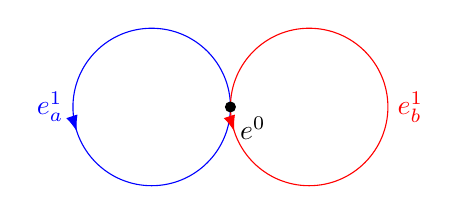
\begin{tikzpicture}[scale=1]
  \draw[blue, midarr] (-1,0) circle (1);
  \draw[red, midarr] (1,0) circle (1);
  \node[blue,left] at (-2,0) {$e^1_a$};
  \node[red,right] at (2,0) {$e^1_b$};
  \fill (0,0) circle (2pt) node[below right] {$e^0$};
\end{tikzpicture}
\end{document}
